\documentclass[letter,12pt]{article}
\usepackage[utf8]{inputenc}
\usepackage[margin=1in]{geometry}

% \usepackage{tikz}
\usepackage{graphicx}
\usepackage{wrapfig}
\usepackage{booktabs}

\usepackage{microtype}
\usepackage{lmodern}

\usepackage{mathtools}

\usepackage{amssymb}
\usepackage{textcomp}
\usepackage{siunitx}

\usepackage[parfill]{parskip}
\usepackage{array}
% \usepackage{multirow}

\newcommand{\tlambda}{\(\lambda\) }
\newcommand{\ttheta}{\(\theta\) }

\sisetup{
  separate-uncertainty,
  multi-part-units = brackets,
  bracket-numbers,
  sticky-per
}
\numberwithin{equation}{section}
\numberwithin{figure}{section}
\numberwithin{table}{section}
\graphicspath{ {./images/} }

\title{Experiment 9 --- Finding the speed of light with microwave optics}
\author{Laurence Amadeus Tristan, Nero Su}
\date{15 March 2019}

\begin{document}
\maketitle

\section{Introduction}
The aim of this experiment is to find the speed of light in air using three different methods of getting the wavelength \tlambda of the microwave source (\(f = \SI{10.525}{\giga\hertz}\)). We then compare the three values of the speed of light in air from those methods in terms of the precision and accuracy of those values.

We define the value of the speed of light in air \(v\) as:
\[ v_a = \SI{3.0}{\metre\per\second} \ \text{(to 1 d.p.)}. \]

\begin{figure}[!ht]
  \centering
  
\includegraphics[width=\textwidth]{goniometer.pdf}
  \caption{A goniometer with the mounted microwave transmitter-receiver pair.}
  \label{fig:i1}
\end{figure}

We use a microwave transmitter-receiver pair mounted on a goniometer (Figure \ref{fig:i1}). The goniometer allows us to change (and measure) the angle of the receiver relative to the transmitter, and both transmitter and receiver's polarization axes are adjustable. The transmitter emits a microwave polarized along the transmitter's axis, and similarly the receiver receives the microwave polarized to its axis.

The plate-holder is an attachment point for the construction of a double-slit plate or a single-slit plate. The plates were stuck together using magnets, which then will be attached to the plate-holder. \pagebreak[4]

Once \tlambda is established using the three experiments, we use the equation
\begin{equation} \label{eq:i1}
  v = f \lambda
\end{equation}
to get a value for the speed of light in air (indicated by \(v\)) for each experiment.

\section{Experiment}
\subsection{Part I: Finding factors affecting intensity of microwaves}
First, we try to figure out what factors affects the intensity of the microwave energy that the receiver detects. We found that the following factors affect the intensity of microwave:

\begin{enumerate}
  \item Distance between the transmitter and receiver. The further the distance, the lower the intensity of microwave received by the receiver. The opposite is true when the distance is decreased.
  \item Relative angle of the polarization axes of the transmitter and receiver. As the receiver turns, the intensity decreases to zero as it approaches \SI{90}{\degree} and increases to its maximum as it approaches \SI{180}{\degree}.
  \item Presence of water between transmitter and receiver. When we put a dry towel between the pair intensity remains the same. However when we placed a wet towel between the pair the microwave is absorbed by the water present in the towel, so the intensity decreases to zero.
\end{enumerate}

\subsection{Part II: Measuring the wavelength \tlambda of microwaves}
For each experiment, we adjust the goniometer such that the angle reads \SI{180}{\degree} for the receiver.

\subsubsection{Standing waves method}
First, move the receiver and the transmitter on the goniometer such that the receiver is at the intensity maxima. Then, make note of the location of the receiver on the ruler. Afterwards, move the receiver towards the transmitter slowly while counting the number of intensity maxima (\(\Delta m\)). Stop moving the receiver at one of the intensity maxima and make note of the location of the receiver and the number of intensity maxima.

\begin{table}[!ht]
  \centering
  \begin{tabular}{cS}
    \toprule
    {\(m\)} & {\(d_m\)/\(\pm 0.1\) \si{\cm}} \\ \midrule
    0 & 93.4 \\
    4 & 87.5 \\
    \bottomrule
  \end{tabular}
  \caption{Initial and final values of the location of the receiver.}
  \label{table:e1}
\end{table}

The relationship between \tlambda and \(d\) is

\begin{equation} \label{eq:e1}
  d = \Delta m \left( \frac{\lambda}{2} \right)
\end{equation} 
\nopagebreak[4]
\begin{tabbing}
  where \= \(\Delta m\) \= = number of intensity maxima, \\
  \> \(d\) \> = difference in location of receiver, \\
  \> \tlambda \> = wavelength of microwave.
\end{tabbing}

Now, get the values for \(\Delta m\) and \(d\). The uncerntainty for \(d\) accumulates as we add/subtract so it'll not be shown as it is trivial enough to do.
\begin{align*}
  \Delta m &= 4 - 0 \\
  &= 4 \\
  d &= d_4 - d_0 \\
  &= \SI{93.4(1)}{\cm} - \SI{87.5(1)}{\cm} \\
  &= \SI{5.9(2)}{\cm}
\end{align*}
Using \eqref{eq:e1}, get the value for the wavelength \tlambda.
\begin{align*}
  \begin{split}
    \SI{5.9}{\cm} &= \frac{(4) \lambda}{2} \\
    \lambda &= \frac{2(\SI{5.9}{\cm})}{4} \\
    &= \SI{2.95}{\cm}
  \end{split}
  \begin{split}
    \delta \lambda &= |\lambda|\left( \frac{\delta d}{d} \right) \\
    &= \SI{2.95}{\cm} \left( \frac{\SI{0.2}{\cm}}{\SI{5.9}{\cm}} \right) \\
    &= \SI{0.1}{\cm}
  \end{split}
\end{align*}
\[\therefore \lambda = \SI{3.0(1)}{\cm}\]

Convert \tlambda to metre and find the value for the speed of light in air \(v\).
\begin{align*}
  \begin{split}
    v &= f \lambda \\
    &= (\SI{10.525e9}{\hertz})(\SI{3.0e-2}{\m}) \\
    &= \SI{3.1575e8}{\m\per\s}
  \end{split}
  \begin{split}
    \delta v &= |v| \left( \frac{\delta \lambda}{\lambda} \right) \\
    &= |\SI{3.1575e8}{\m}| \left( \frac{\SI{1e-3}{\m}}{\SI{3.0e-2}{\m}} \right) \\
    &= \SI{1.07034e7}{\m\per\s} \\
    &\approx \SI{1e7}{\m\per\s} \ \text{(to 1 s.f.)}
  \end{split}
\end{align*}
\[\therefore v = \SI{3.2(1)e8}{\m\per\s}\]

\subsubsection{Double-slit inteference method}
\begin{figure}
  \centering
  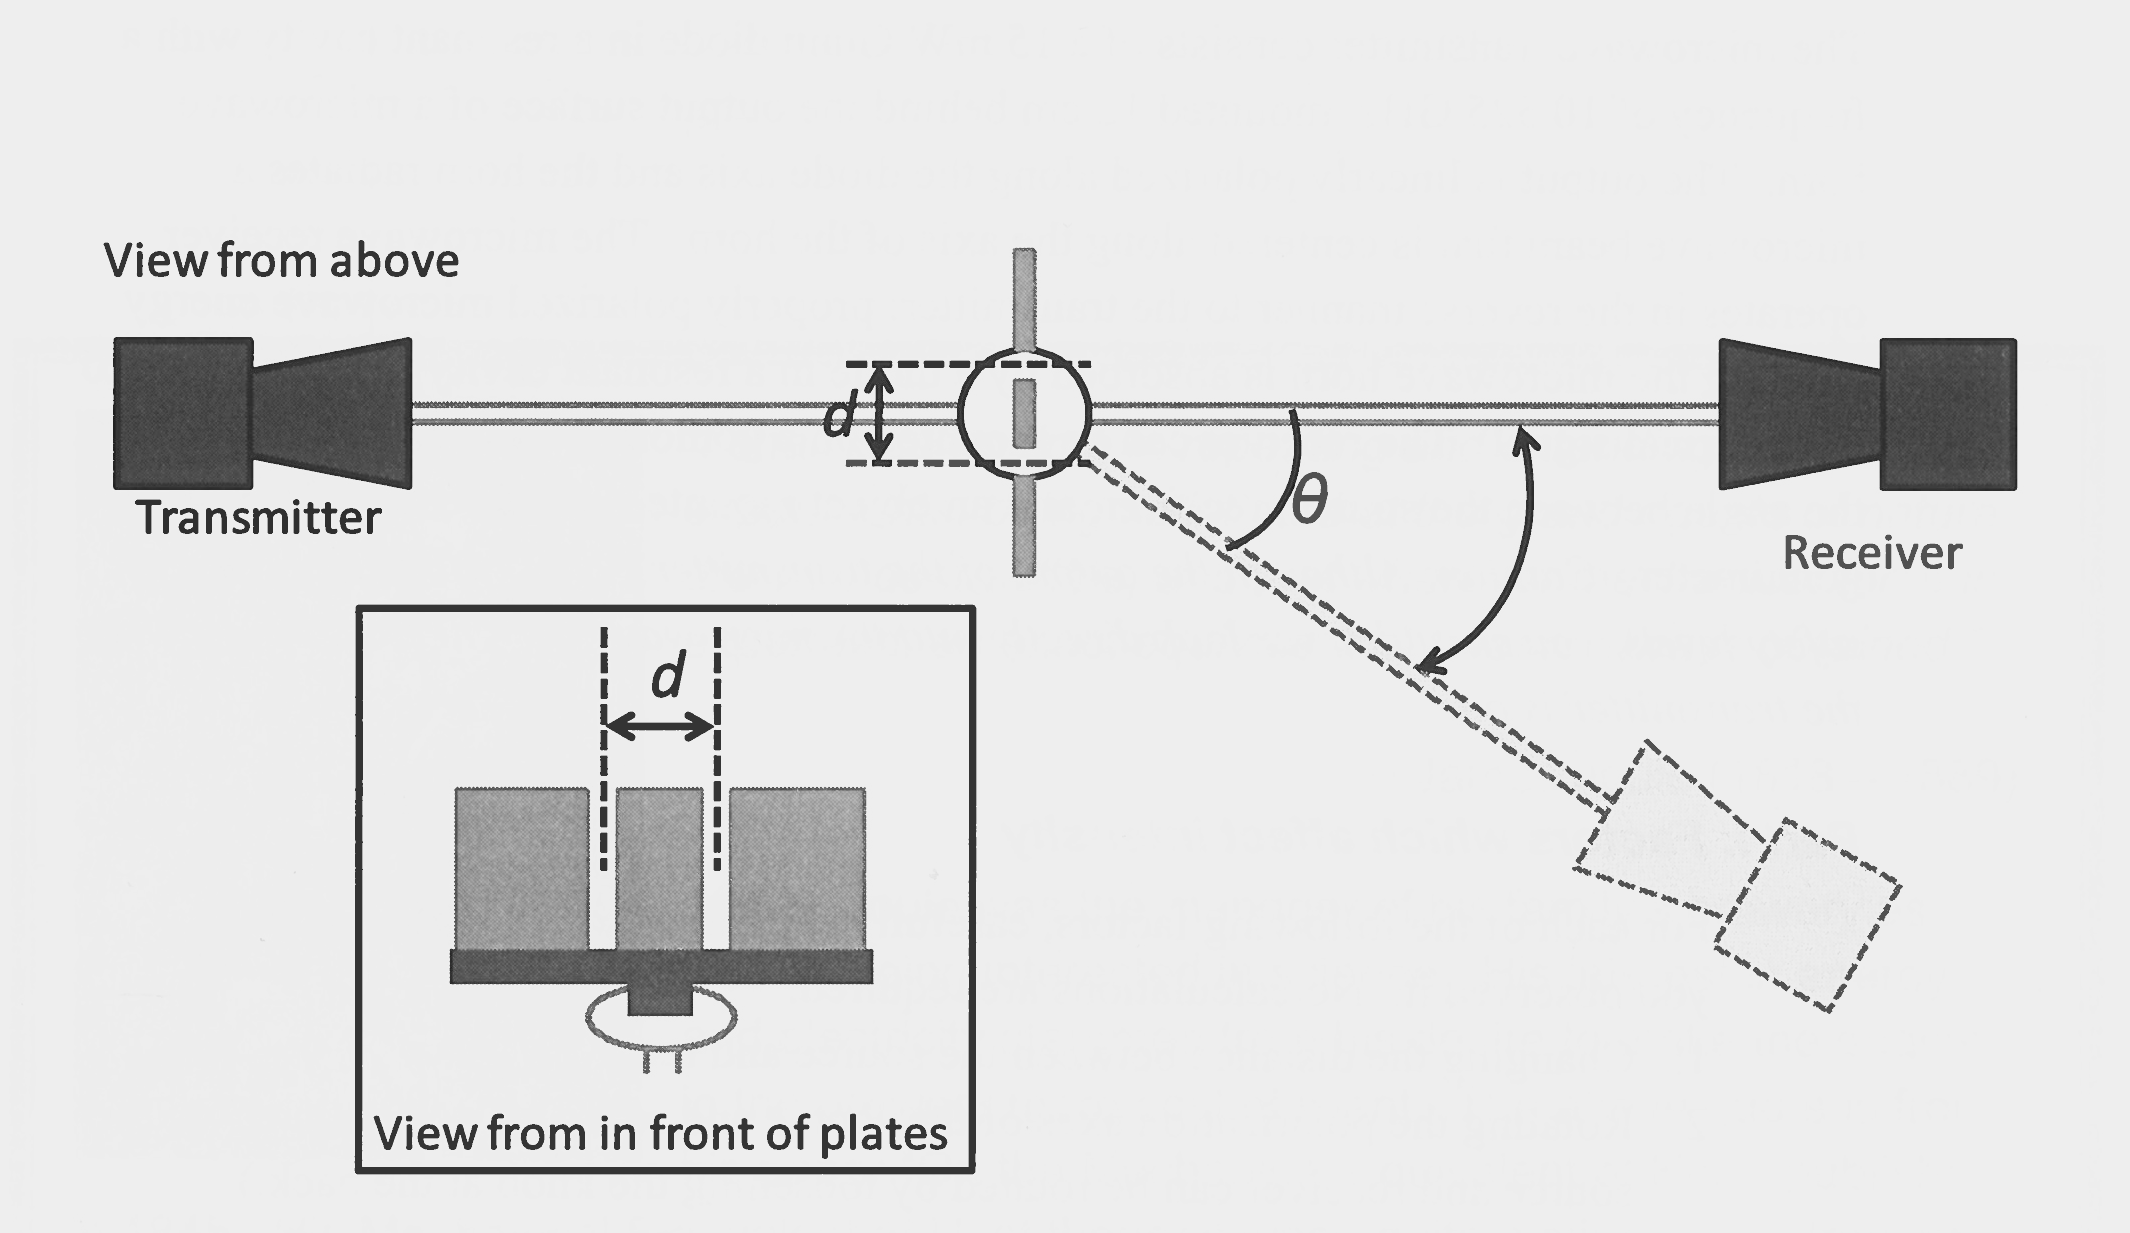
\includegraphics[width=\textwidth]{Double-slit.png}
  \caption{Apparatus setup for the double-slit inteference experiment.}
  \label{fig:e1}
\end{figure}
Setup the apparatus as shown in Figure \ref{fig:e1}. It is suggested to move the transmitter as close to the plate as possible, while adjusting the receiver such that it is located in one of the intensity maxima. Then, using the available plates construct a double-slit, with the width of the slit each being \SI{2}{\cm}, and a slit spacing (denoted as \(d\)) of about \SI{8}{\cm}, measured centre to centre. Make sure the slits are aligned as symmetrical as possible, and the individual slits as vertical as possible. Now, rotate the receiver arm slowly to find the first diffraction maximum. If necessary, move the arm the other way around to confirm the angle between the centre and the first diffraction maximum.

\begin{table}[!ht]
  \centering
  \begin{tabular}{cS}
    \toprule
    {Variable} & {Value} \\ \midrule
    \(\theta_0\) & \SI{180}{\degree} \\
    \(\theta_1\) & \SI{159(2)}{\degree} \\
    \(d\) & \SI{8.0(2)}{\cm} \\
    \bottomrule
  \end{tabular}
  \caption{Data gathered from the double-slit experiment.}
  \label{table:e2}
\end{table}

Before continuing with the calculation, we need to get the expression for the uncertainty of \(\sin{} \theta\). First, let's define \(\sin \theta\) in terms of \(z\).
\begin{align*}
  z &= \sin \theta \\
  \frac{d}{d\theta}(z) &= \cos \theta 
\end{align*}

Now, for a value of \(z\), the uncertainty of \(z\) (and hence \(\sin \theta \)) is
\begin{align} \label{eq:e2}
  \delta z &= \frac{d}{d \theta}(z) \  \delta \theta \notag \\
  \delta (\sin \theta) &= \cos \theta \ \delta \theta.
\end{align}

Get the values for \ttheta and convert \(\delta\theta\) to radians.
\begin{align*}
  \theta &= \SI{180}{\degree} - \SI{159(2)}{\degree} \\
  &= \SI{21(2)}{\degree} \\
  \delta \theta \ (\mathrm{radians}) &\approx 0.0349065850398866 \ (\text{16 s.f.})
\end{align*}

Using \[\lambda = d \sin \theta,\] find the value for \tlambda using values obtained from the double-slit experiment.
\begin{align*}
  \begin{split}
    \lambda &= d \sin \theta \\
    &= (\SI{8.0}{\cm}) \sin{\SI{21}{\degree}} \\
    &\approx \SI{2.866944}{\cm} \ \text{(6 d.p.)}
  \end{split}
  \begin{split}
    \delta \lambda &= |\lambda| \left( \frac{\delta d}{d} + \frac{\delta (\sin\theta)}{\sin \theta} \right) \\
    &= |(\SI{8.0}{\cm}) \sin{\SI{21}{\degree}}| \left( \frac{\SI{0.2}{\cm}}{\SI{8.0}{\cm}} + \frac{(\cos{\SI{21}{\degree}})(0.03490658\dots)}{\sin{\SI{21}{\degree}}} \right) \\
    &\approx \SI{0.332378}{\cm} \ \text{(to 6 d.p.)} \\
    &\approx \SI{0.3}{\cm} \ \text{(1 s.f.)}
  \end{split}
\end{align*}
\[\therefore \lambda = \SI{2.9(3)}{\cm}\]

Convert \tlambda to metre and find the value for \(v\) (using \eqref{eq:i1}).
\begin{align*}
  \begin{split}
  v &= f \lambda \\
  &= (\SI{10.525(9)}{\hertz})(\SI{0.029(3)}{\m}) \\
  &= \SI{3.05225e8}{\metre\per\second}
  \end{split}
  \begin{split}
    \delta v &= |v|\left( \frac{\delta \lambda}{\lambda} \right) \\
    &= |\SI{3.05225e8}{\metre\per\second}|\left( \frac{\SI{0.003}{\m}}{\SI{0.029}{\m}} \right) \\
    &= \SI{3.15755e7}{\m\per\s} \\
    &\approx \SI{3e7}{\m\per\s}
  \end{split}
\end{align*}
\[\therefore v = \SI{3.1(3)e8}{\m\per\s}\]

\subsubsection{Single-slit inteference method}
\begin{figure}[!ht]
  \centering
  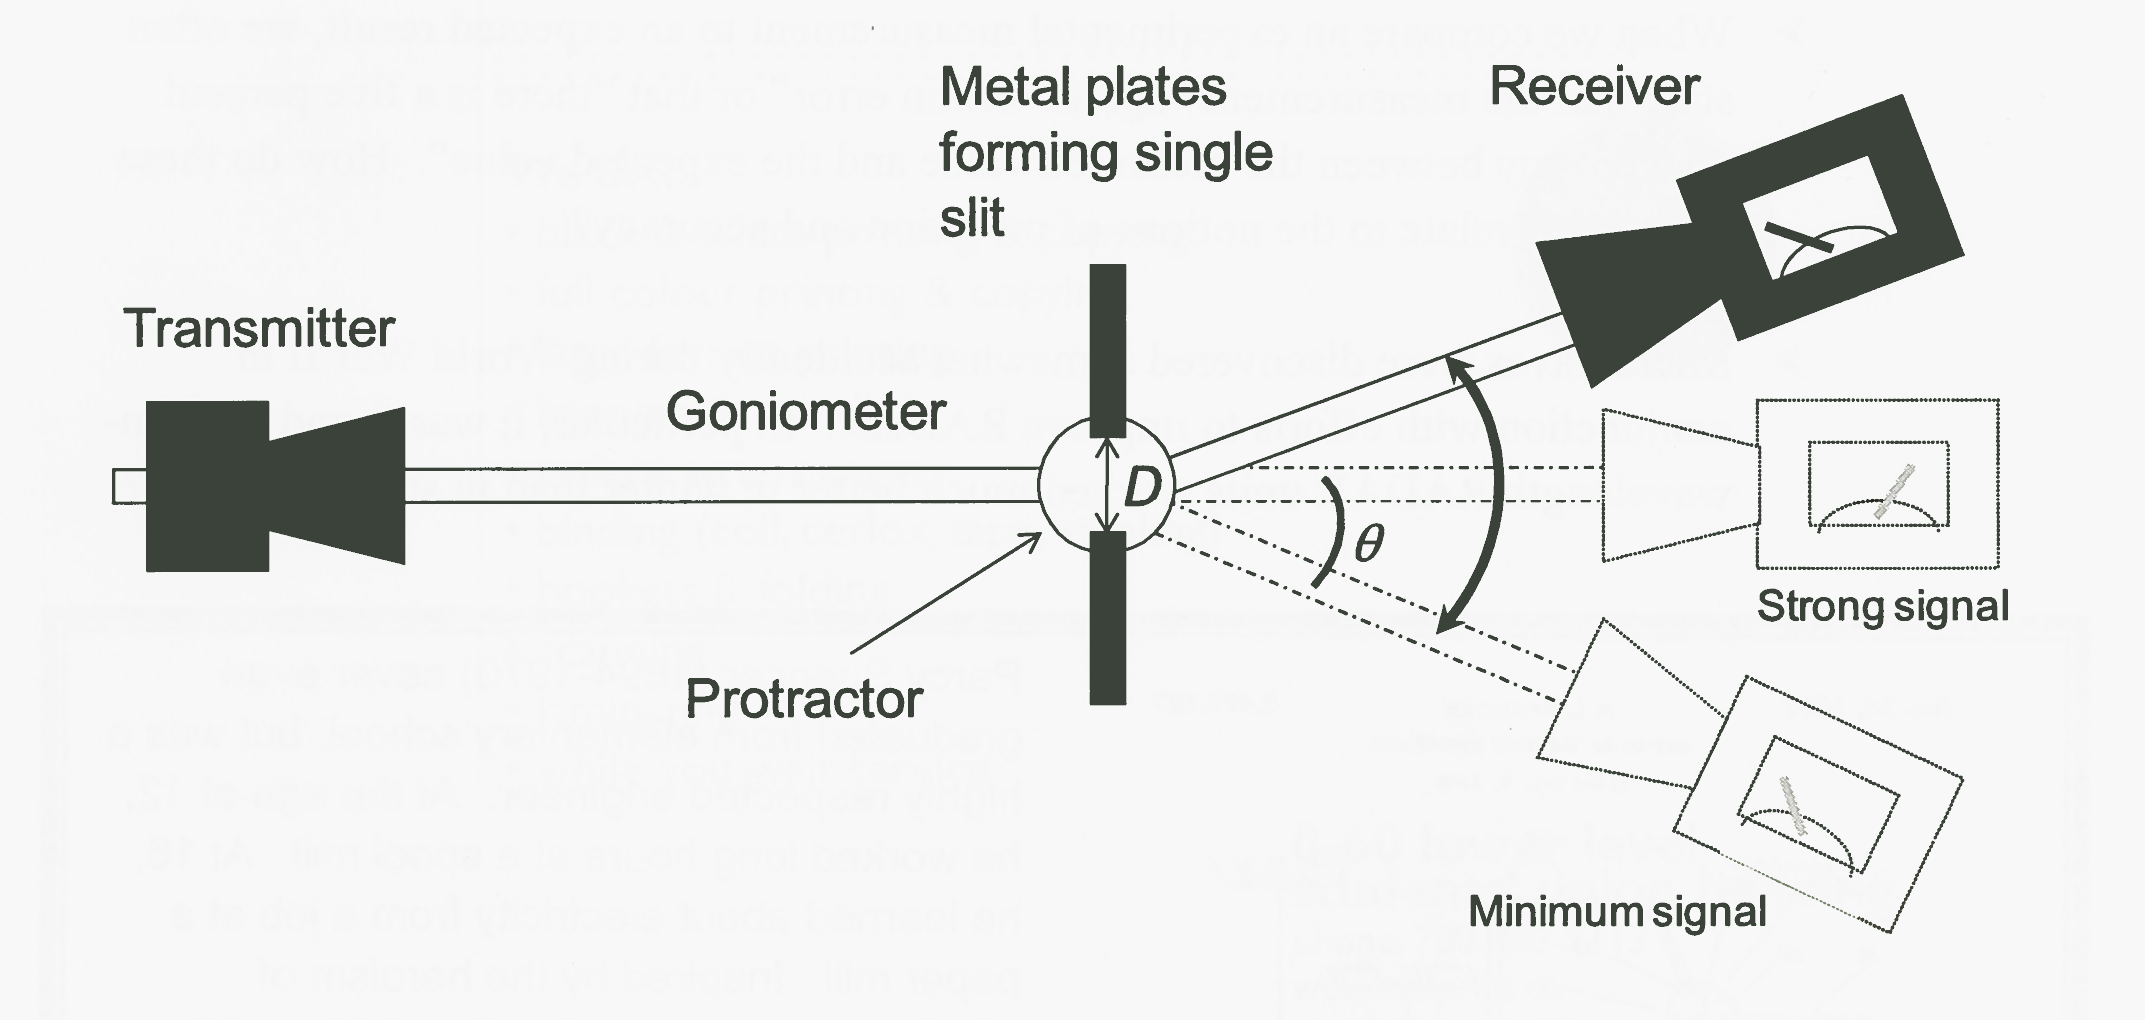
\includegraphics[width=\textwidth]{Single-slit.png}
  \caption{Apparatus setup for the single-slit inteference experiment.}
  \label{fig:e2}
\end{figure}

Setup the apparatus as shown in Figure \ref{fig:e2}. The suggestion for the double-slit inteference experiment still hold for this method. With the available plates, replace the double-slit arrangement with the single slit with the width of the slit \(D\) being around \SIrange{7}{8}{\cm}. Make sure the slit are aligned as symmetrical as possible, and the slit perimeters as close to vertical as possible. Afterwards, start rotating the arm slowly while increasing sensitivity (and if possible, its scale) of the receiver to find the first diffraction \emph{minima}. This will prove difficult, so we highly suggest double-checking the angle \ttheta by rotating it the other way.

\begin{table}[!ht]
  \centering
  \begin{tabular}{cS}
    \toprule
    {Variable} & {Value} \\ \midrule
    \(\theta_0\) & \SI{180}{\degree} \\
    \(\theta_1\) & \SI{161(4)}{\degree} \\
    \(D\) & \SI{7.0(2)}{\cm} \\
    \bottomrule
  \end{tabular}
  \caption{Data gathered from the single-slit experiment.}
  \label{table:e3}
\end{table}

The equation needed for \(\delta(\sin \theta)\) has been derived so we will use the result from Equation \ref{eq:e2}

Get the value for \ttheta and convert \(\delta \theta\) to radians using data from Table \ref{table:e3}.
\begin{align*}
  \theta &= \SI{180}{\degree} - \SI{161(4)}{\degree} \\
  &= \SI{19(4)}{\degree} \\
  \delta \theta \ \text{(radians)} &\approx 0.0698132 \ \text{(6 s.f.)}
\end{align*}

With \[\lambda = D \sin \theta, \] find the value for \tlambda using values from Table \ref{table:e3}.
\begin{align*}
  \begin{split}
    \lambda &= D \sin \theta \\
    &= (\SI{7.0}{\cm}) \sin{\SI{19}{\degree}} \\
    &\approx \SI{2.278977}{\cm} \ \text{(6 d.p.)}
  \end{split}
  \begin{split}
    \delta \lambda &= |\lambda| \left( \frac{\delta D}{D} + \frac{\delta (\sin\theta)}{\sin \theta} \right) \\
    &= |(\SI{7.0}{\cm}) \sin{\SI{19}{\degree}}| \left( \frac{\SI{0.2}{\cm}}{\SI{7.0}{\cm}} + \frac{(\cos{\SI{21}{\degree}})(0.0698132)}{\sin{\SI{19}{\degree}}} \right) \\
    &\approx \SI{0.242691}{\cm} \ \text{(to 6 d.p.)} \\
    &\approx \SI{0.2}{\cm} \ \text{(1 s.f.)}
  \end{split}
\end{align*}
\[\therefore \lambda = \SI{2.3(2)}{\cm}\]

Convert \tlambda to metre and find the value for \(v\) (using \eqref{eq:i1}).
\begin{align*}
  \begin{split}
  v &= f \lambda \\
  &= (\SI{10.525(9)}{\hertz})(\SI{0.023(2)}{\m}) \\
  &= \SI{2.3166e8}{\metre\per\second}
  \end{split}
  \begin{split}
    \delta v &= |v|\left( \frac{\delta \lambda}{\lambda} \right) \\
    &= |\SI{2.3166e8}{\metre\per\second}|\left( \frac{\SI{0.002}{\m}}{\SI{0.023}{\m}} \right) \\
    &= \SI{2.106e7}{\m\per\s} \\
    &\approx \SI{2e7}{\m\per\s}
  \end{split}
\end{align*}
\[\therefore v = \SI{2.3(2)e8}{\m\per\s}\]

\pagebreak
\section{Conclusions}
From this experiment, we were able to use the two properties of waves, interference and diffraction, to determine the wavelength of microwave. The three methods that we used gives a practical example of how waves behave and how it relates to the wavelength of the wave itself.

Looking at the three values of the speed of light in air \(v\), the first method (standing waves method) gives the most precise value of \(v\) due to its low uncertainty, while the double-slit method was the least precise of all. However, when comparing with the ground truth value (\(v_a\)), we found that the although the double-slit method was the least precise, however it gives the most accurate value for \(v\). The standing wave method gave us an answer, while \SI{0.2}{\m\per\s} off, was the second-most accurate; whereas the single-slit diffraction method was the least accurate of all.

We suspect that there might be systematic errors that we did not account for in the experiment, and as such both standing waves and single-slit diffraction methods did not correctly predict the speed of light. Not only that, we might have underestimated the uncertainties of our measurements due to the systematic and random errors that we did not take into account. To improve, one suggestion would be to stay away from the transmitter as our human body absorb microwaves due to its water content.  

\end{document}